\section{Hasil Keluaran Plot RDF dan MSD untuk Setiap Variasi}\
\begin{figure}[H]
  \centering
  \begin{subfigure}{0.9\textwidth}
    \centering
    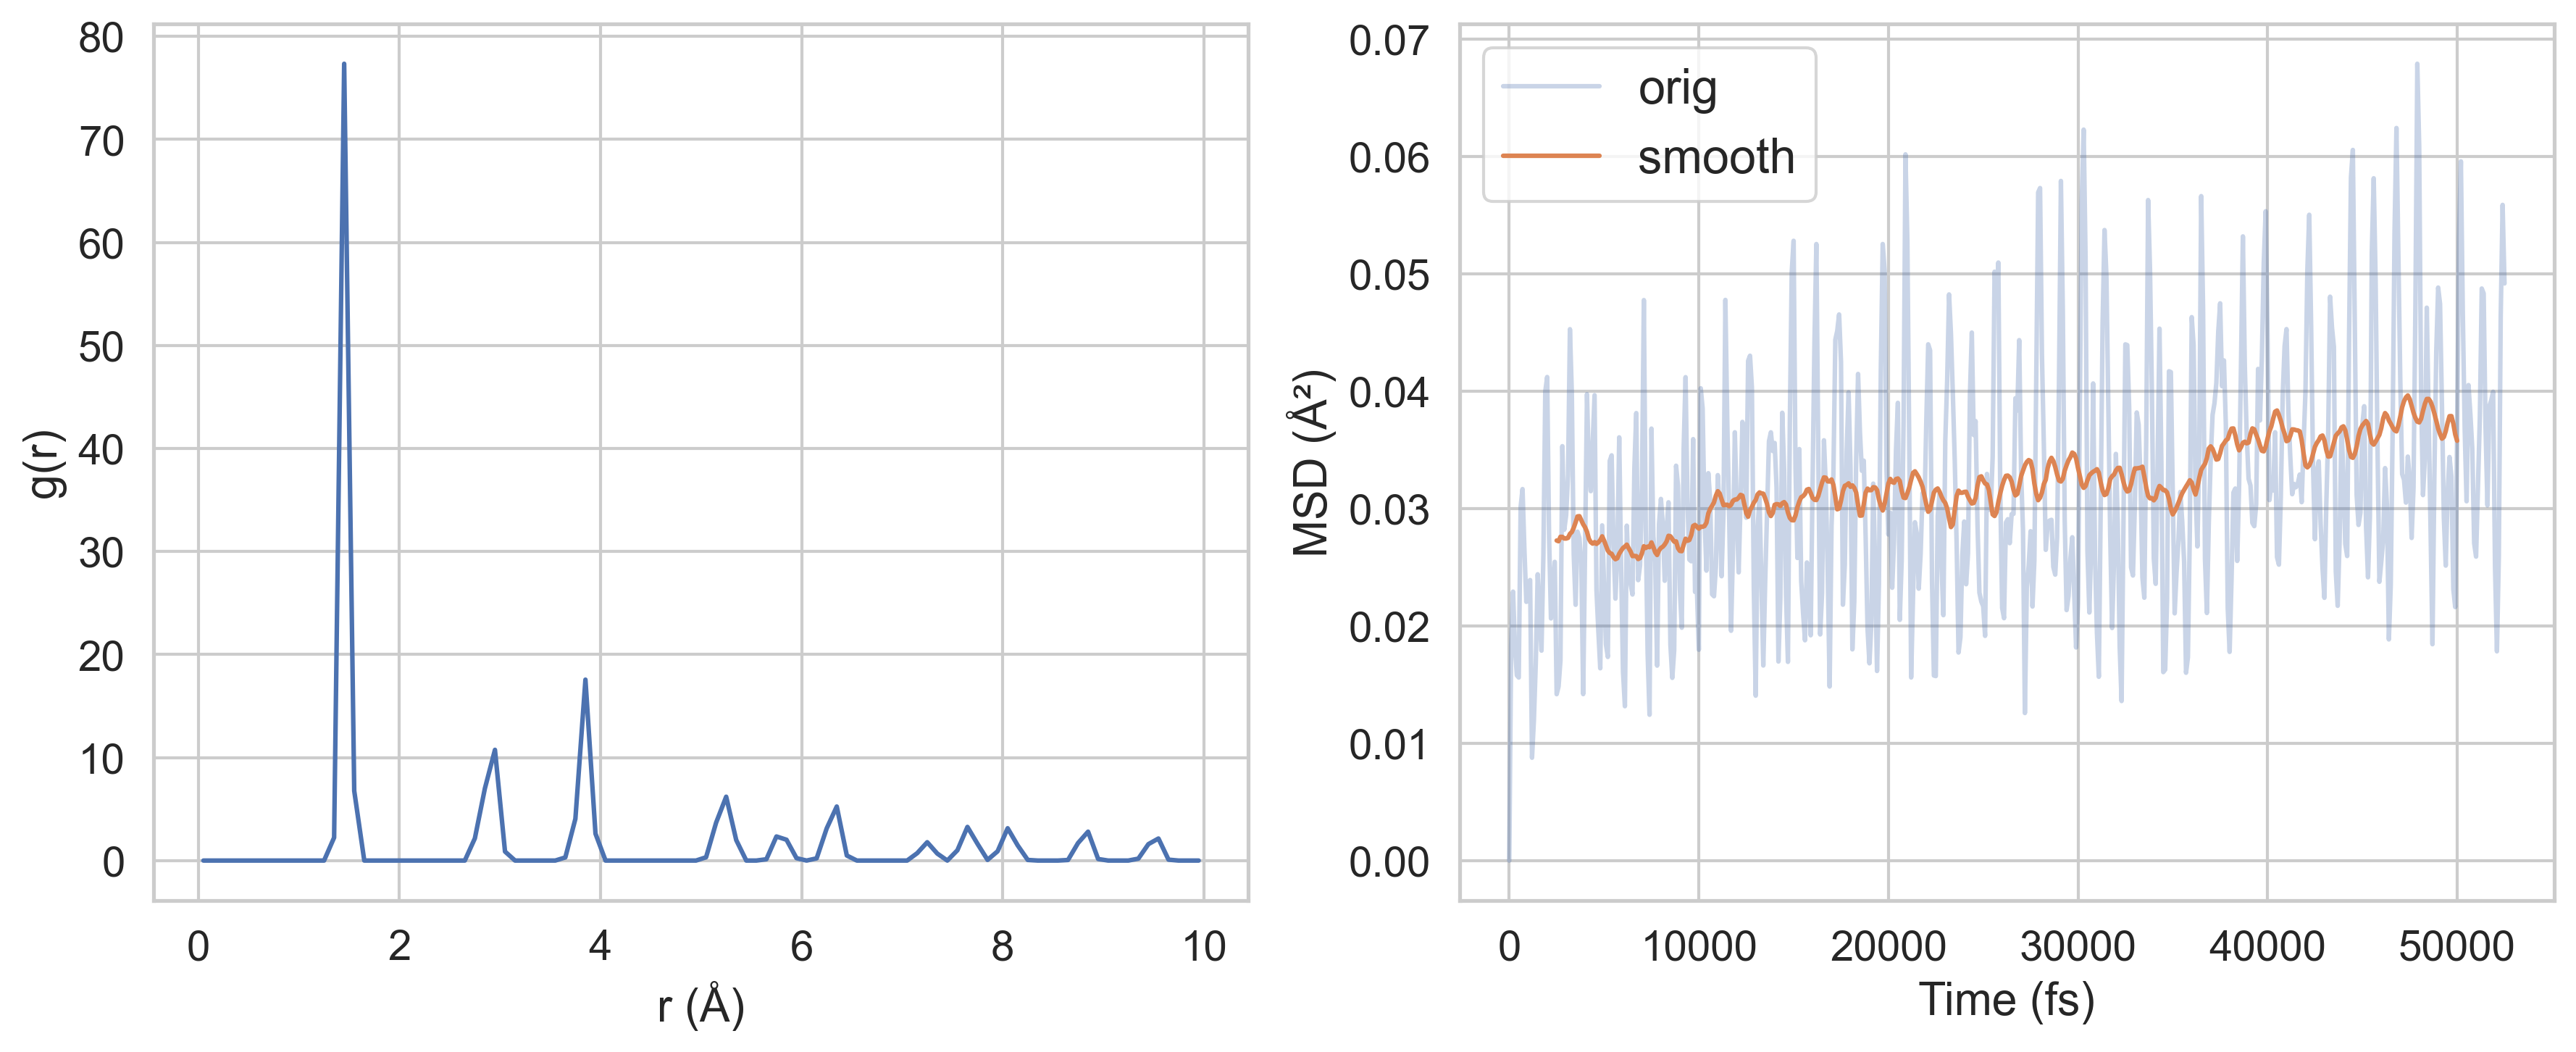
\includegraphics[width=\linewidth]{pure_800K_notitle.png}
    \caption{Murni, 800 K}
    \label{subfig:rdf_msd_pure_800k}
  \end{subfigure}
  \vspace{1em}
  \begin{subfigure}{0.9\textwidth}
    \centering
    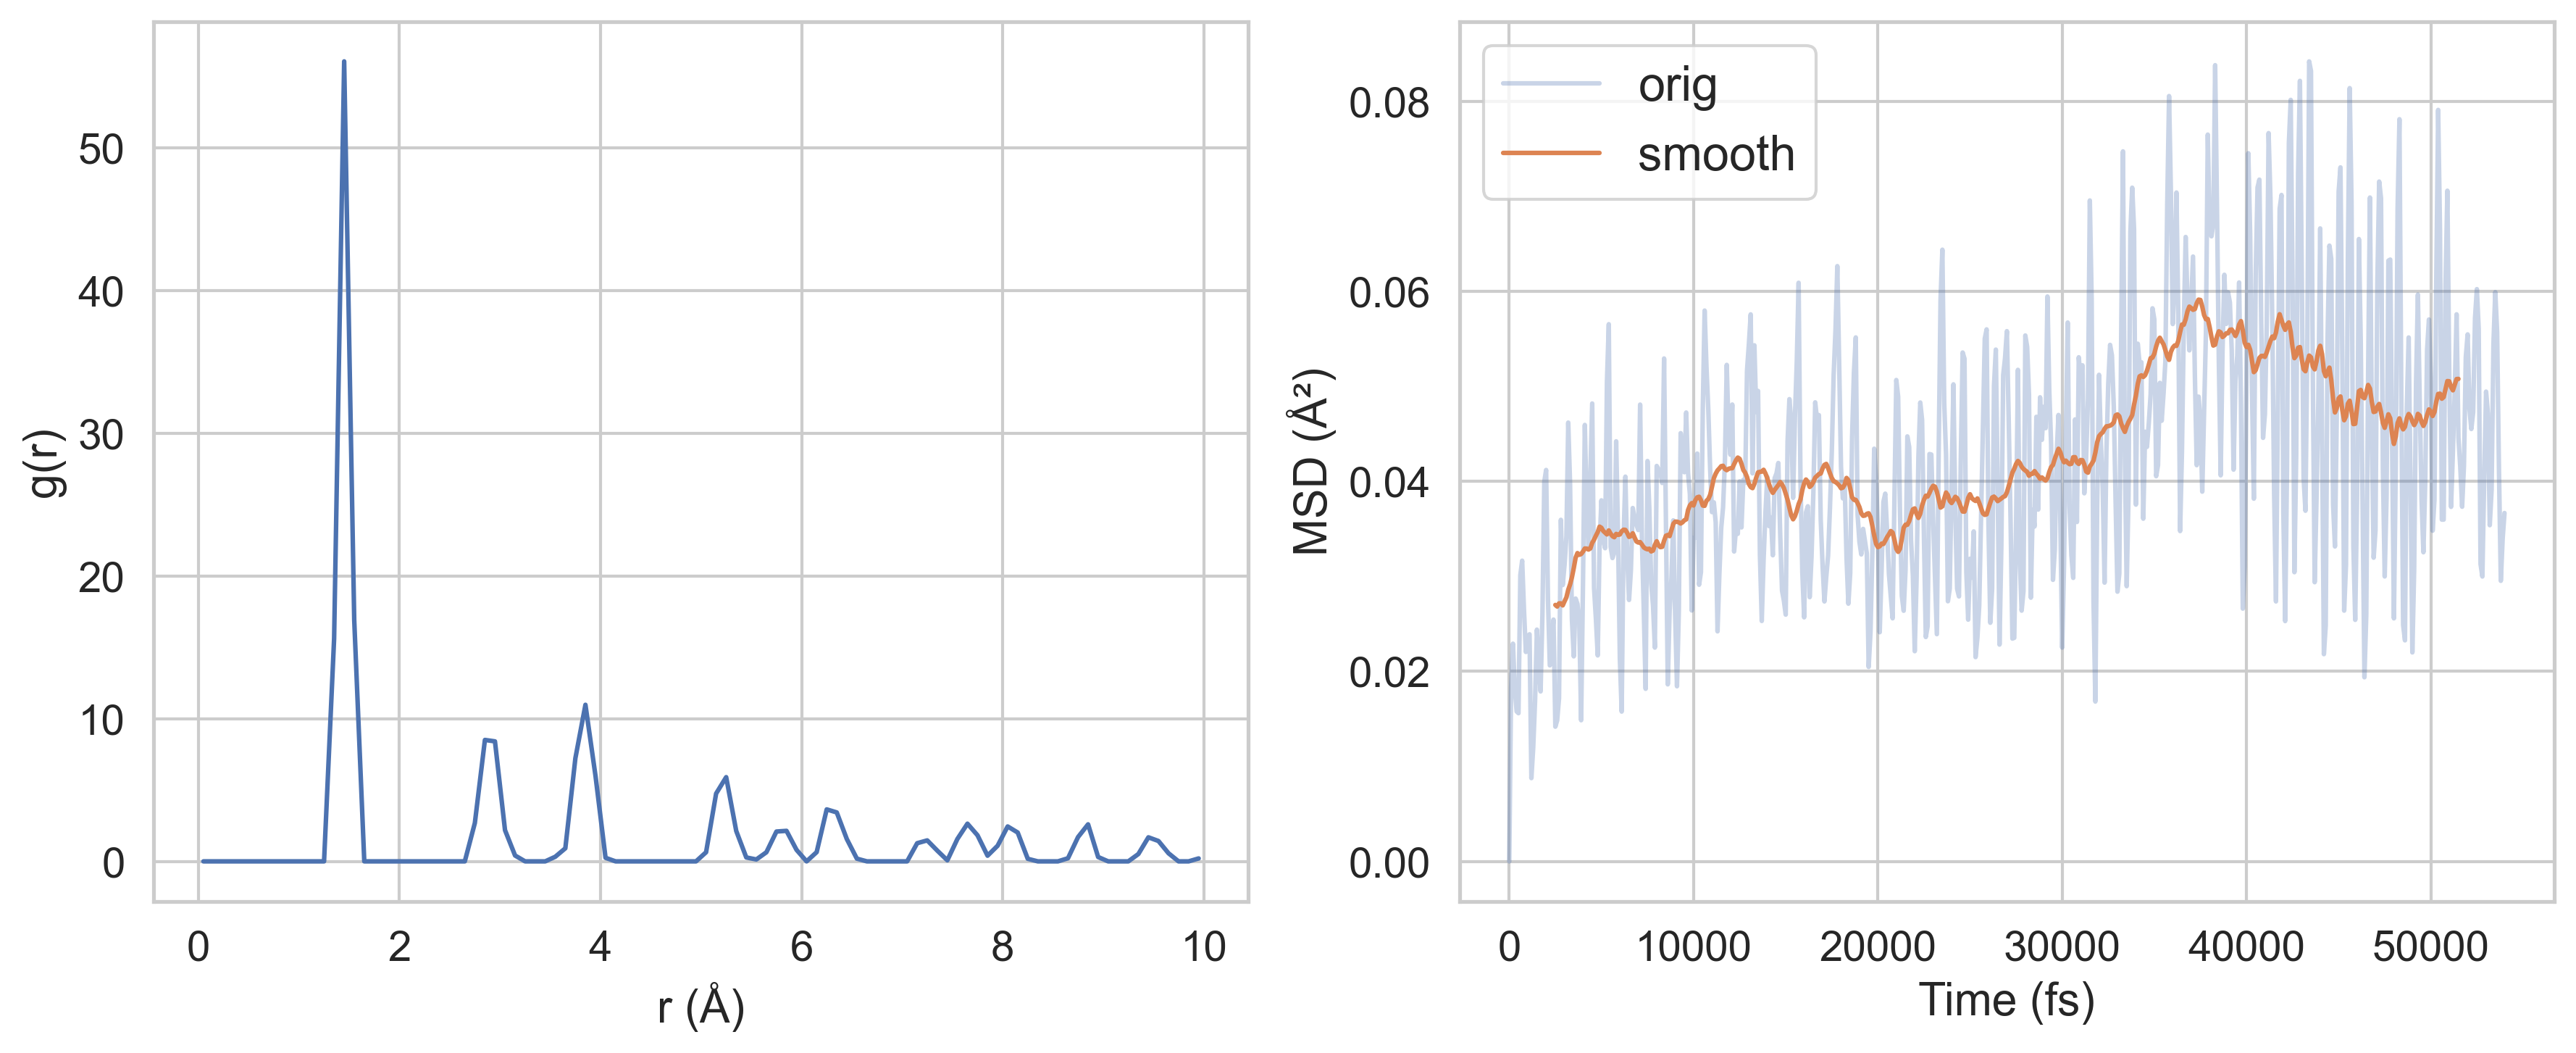
\includegraphics[width=\linewidth]{pure_1100K_notitle.png}
    \caption{Murni, 1100 K}
    \label{subfig:rdf_msd_pure_1100k}
  \end{subfigure}
  \vspace{1em}
  \begin{subfigure}{0.9\textwidth}
    \centering
    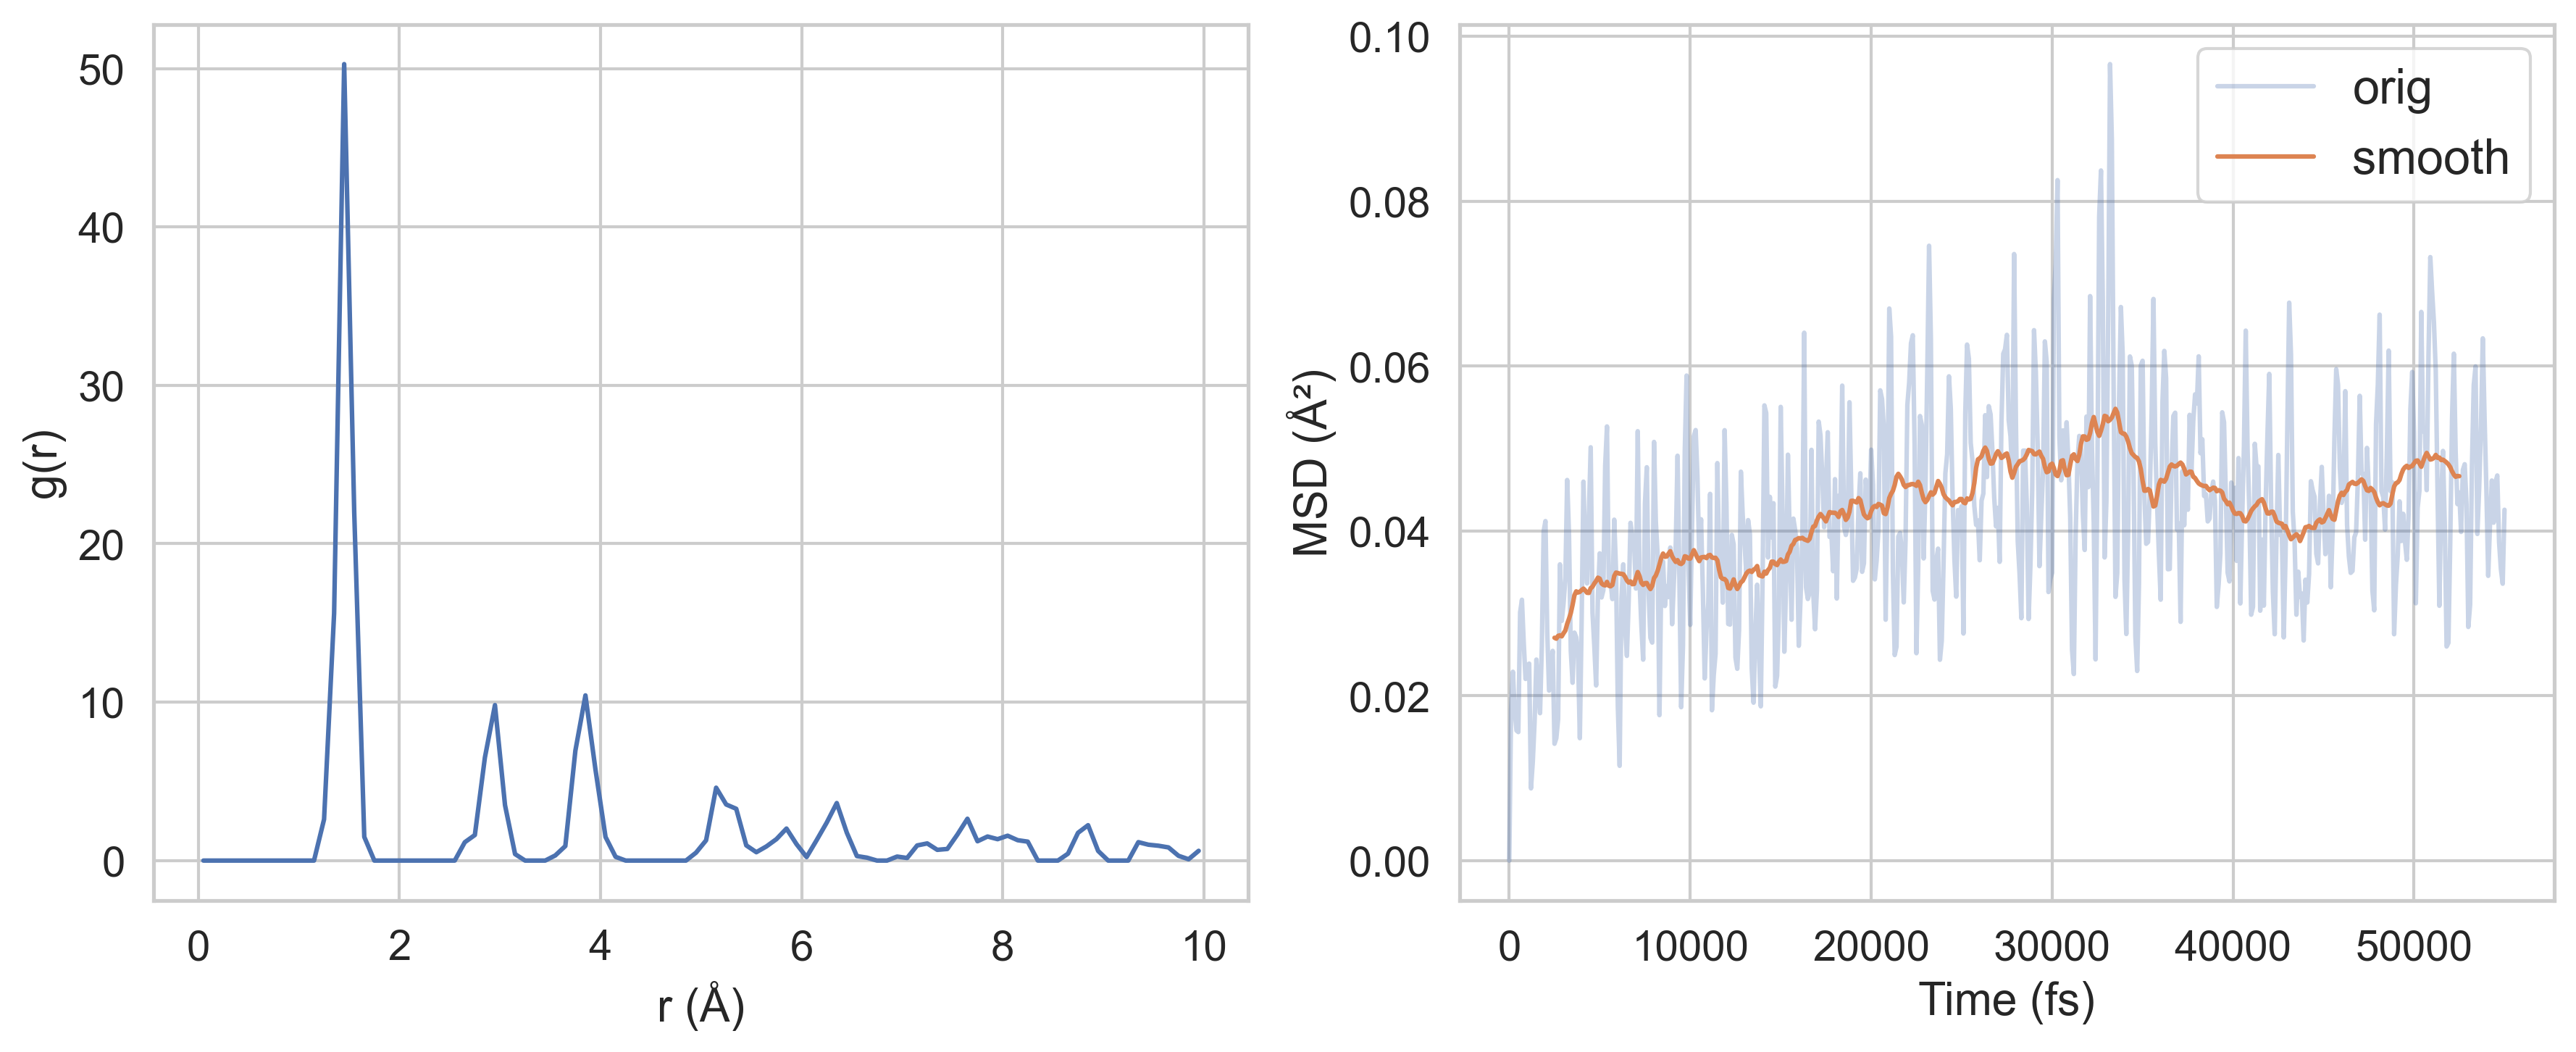
\includegraphics[width=\linewidth]{pure_1225K_notitle.png}
    \caption{Murni, 1225 K}
    \label{subfig:rdf_msd_pure_1225k}
  \end{subfigure}
  \label{fig:rdf_msd_grid}
\end{figure}

% --- Bagian 2: Cacat N_B ---
\begin{figure}[H]\ContinuedFloat
  \centering
  \begin{subfigure}{0.9\textwidth}
    \centering
    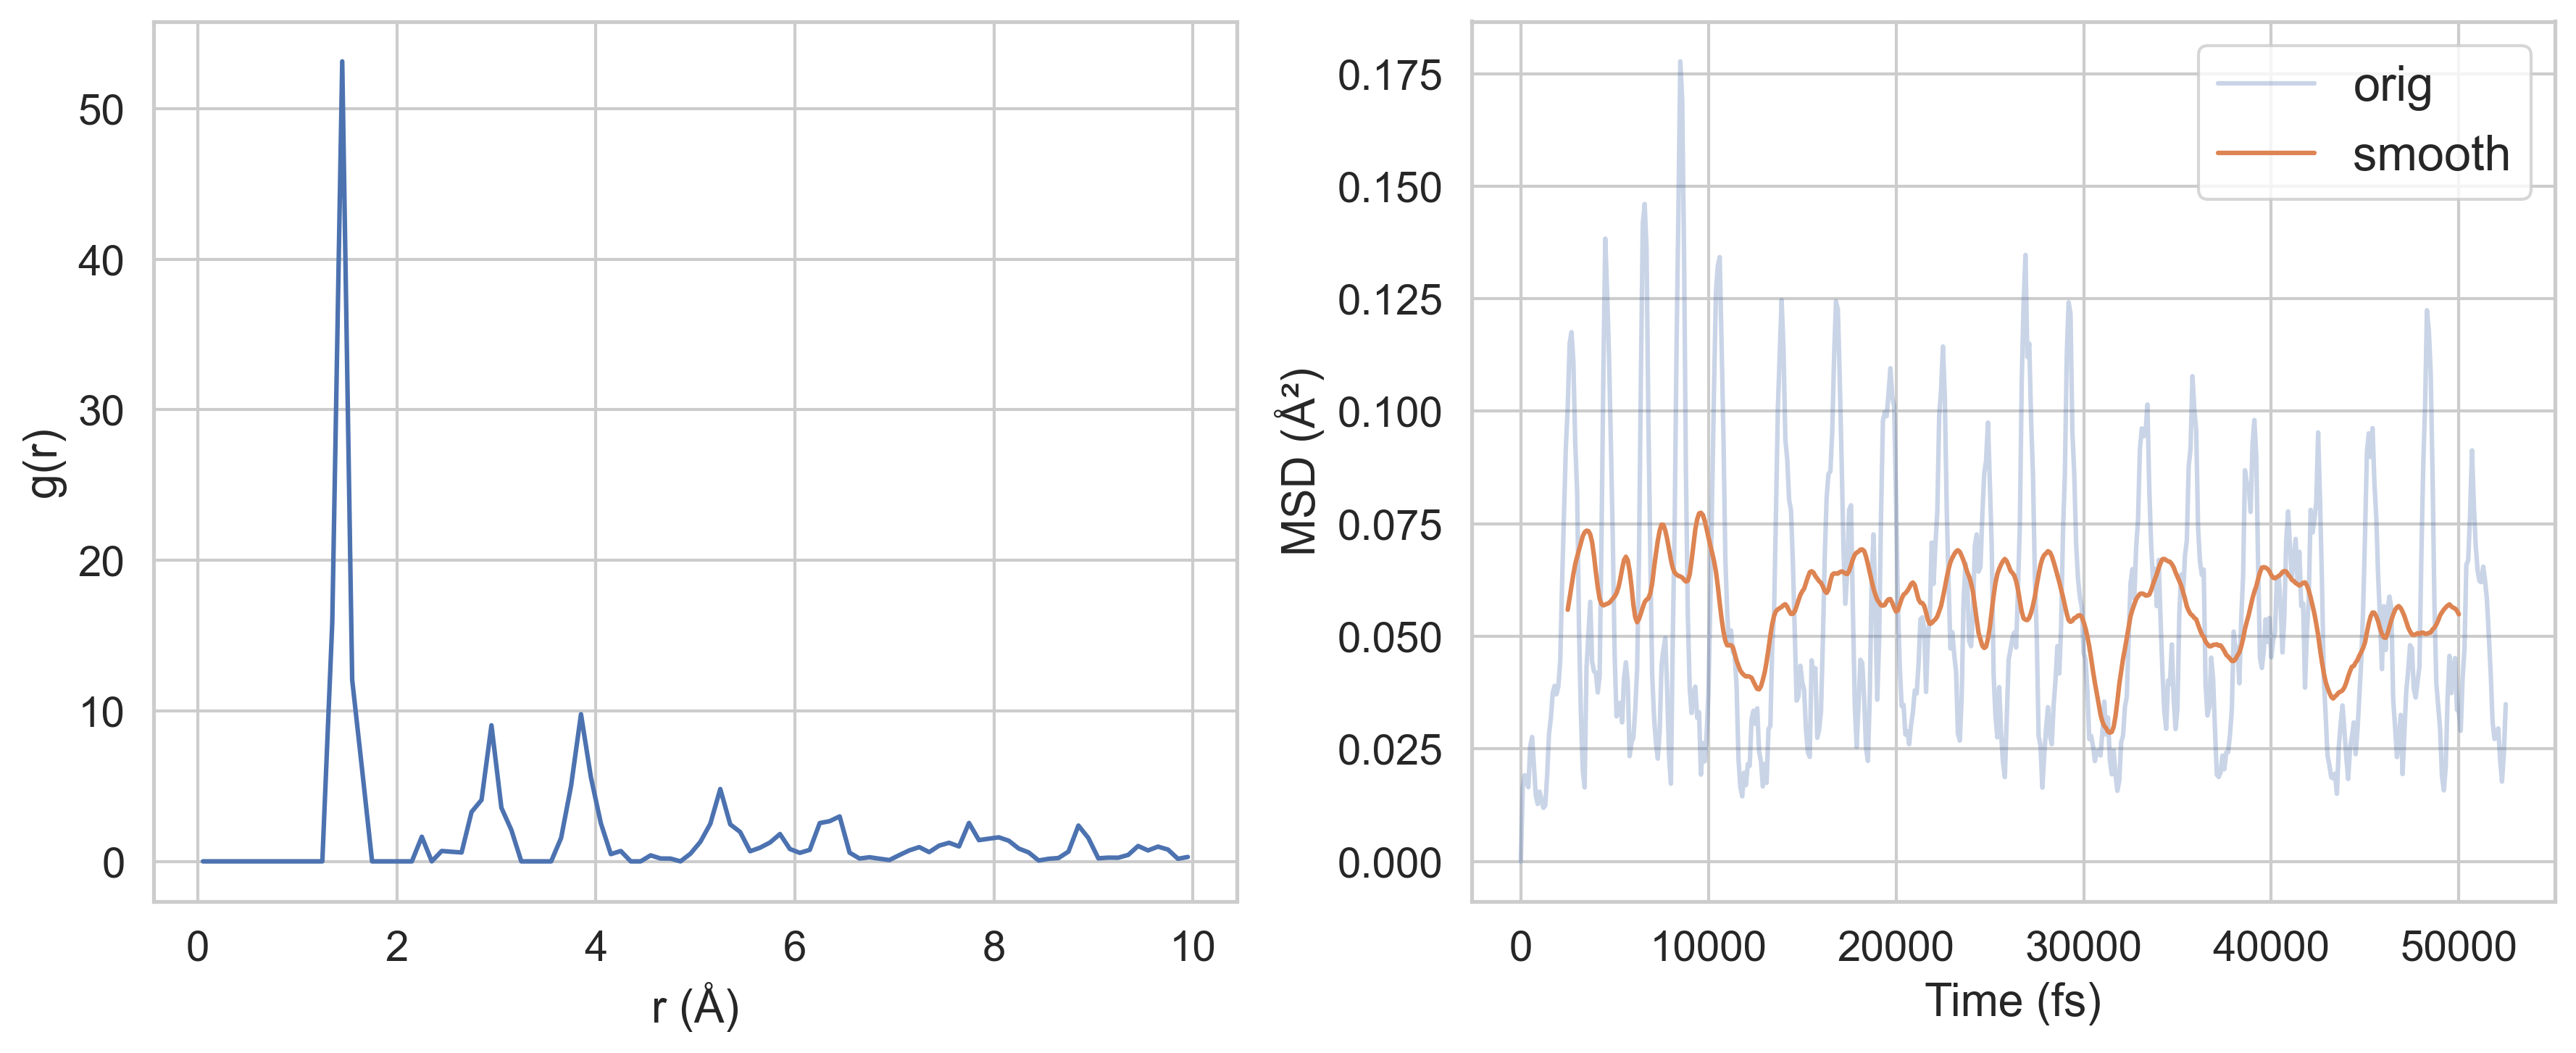
\includegraphics[width=\linewidth]{NN_800K_notitle.png}
    \caption{Cacat N\textsubscript{B}, 800 K}
    \label{subfig:rdf_msd_nn_800k}
  \end{subfigure}
  \vspace{1em}
  \begin{subfigure}{0.9\textwidth}
    \centering
    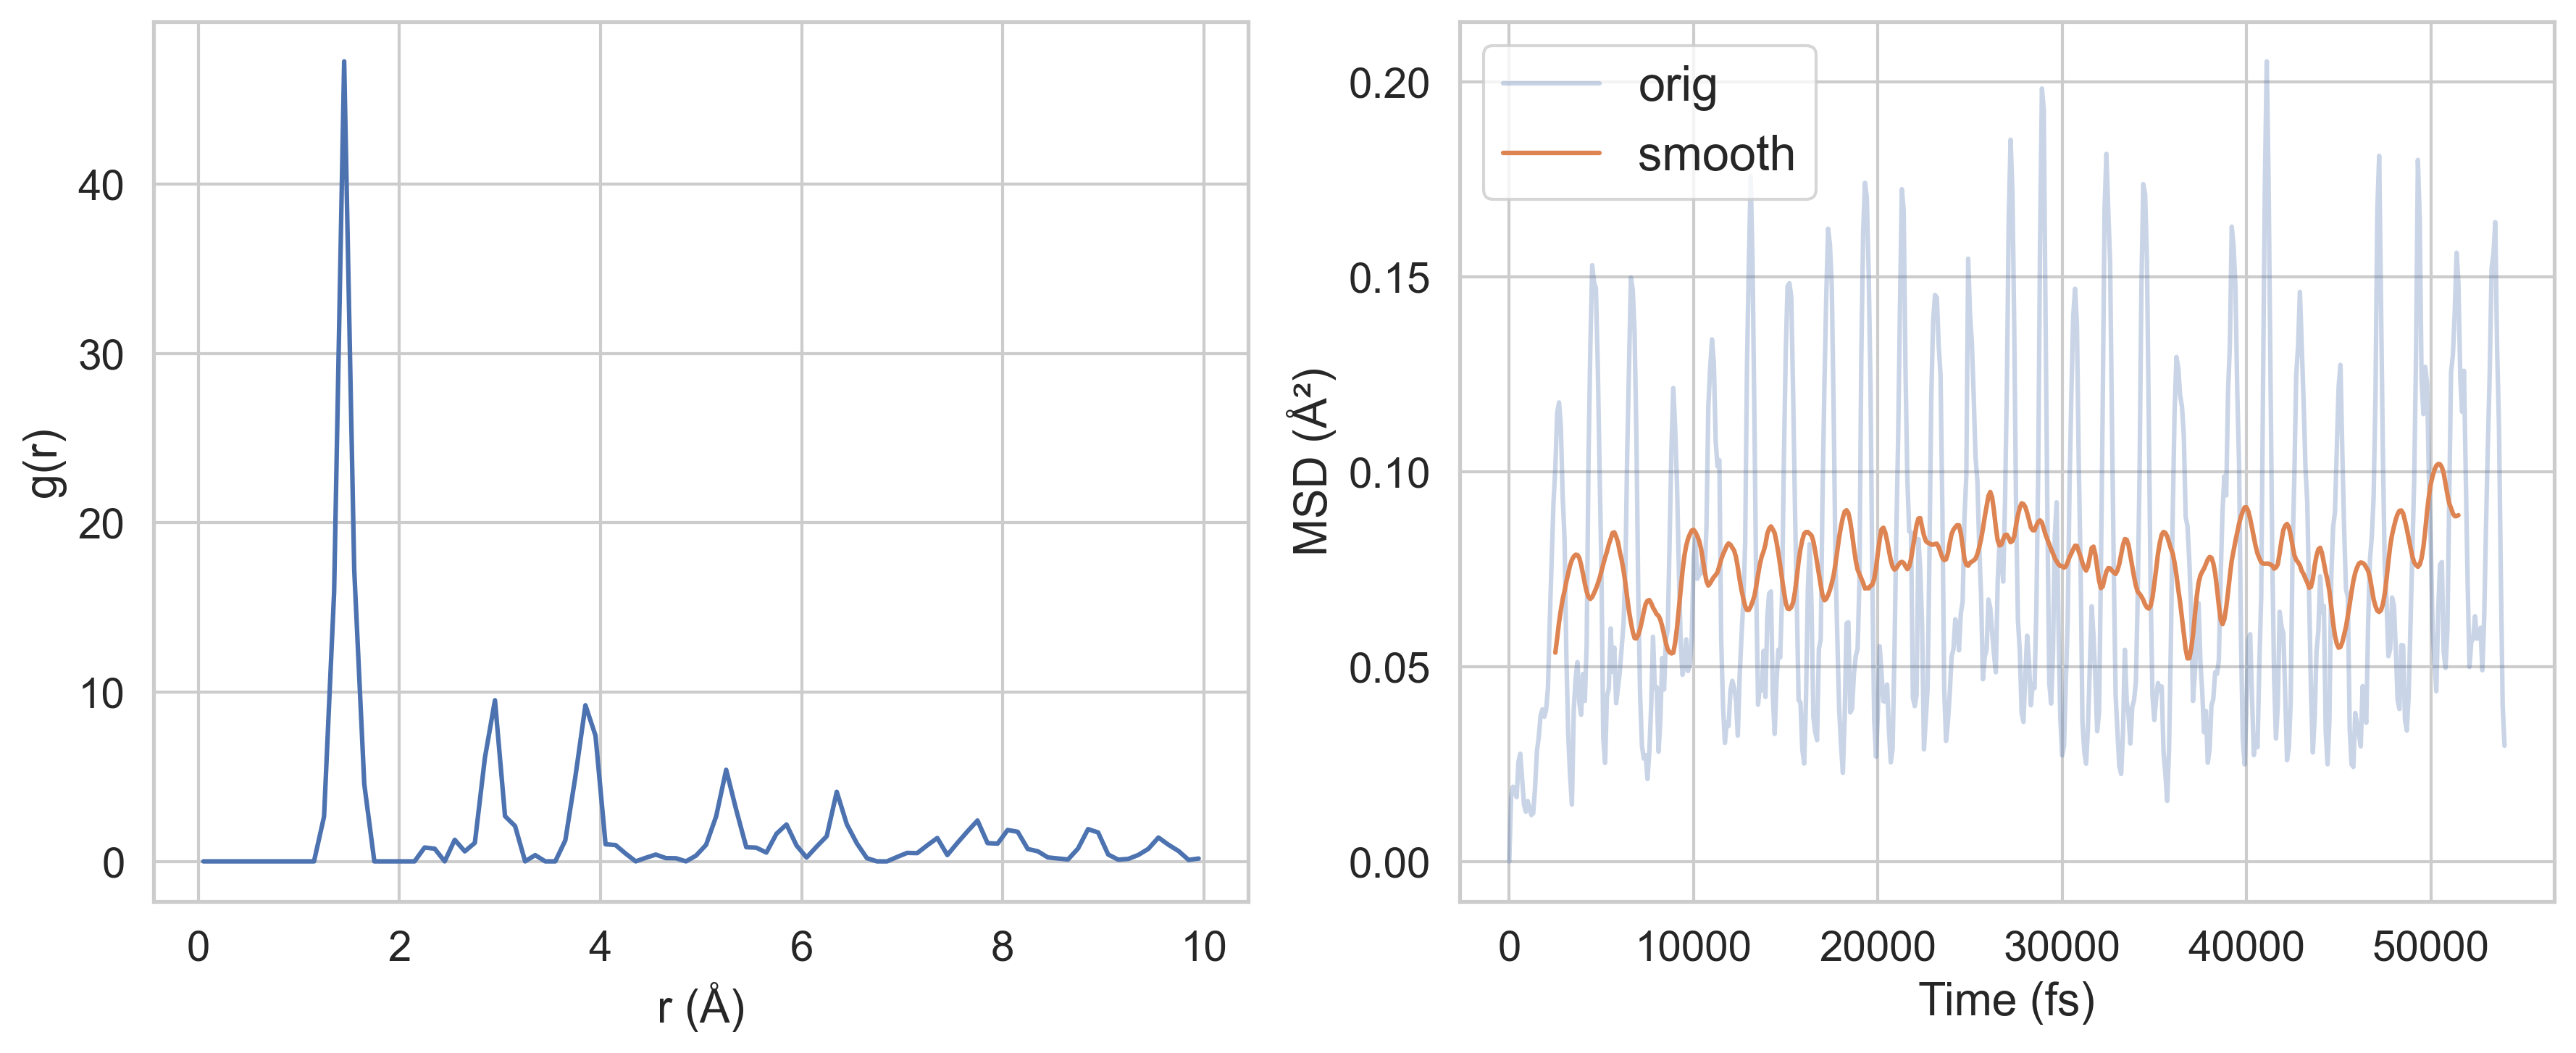
\includegraphics[width=\linewidth]{NN_1100K_notitle.png}
    \caption{Cacat N\textsubscript{B}, 1100 K}
    \label{subfig:rdf_msd_nn_1100k}
  \end{subfigure}
  \vspace{1em}
  \begin{subfigure}{0.9\textwidth}
    \centering
    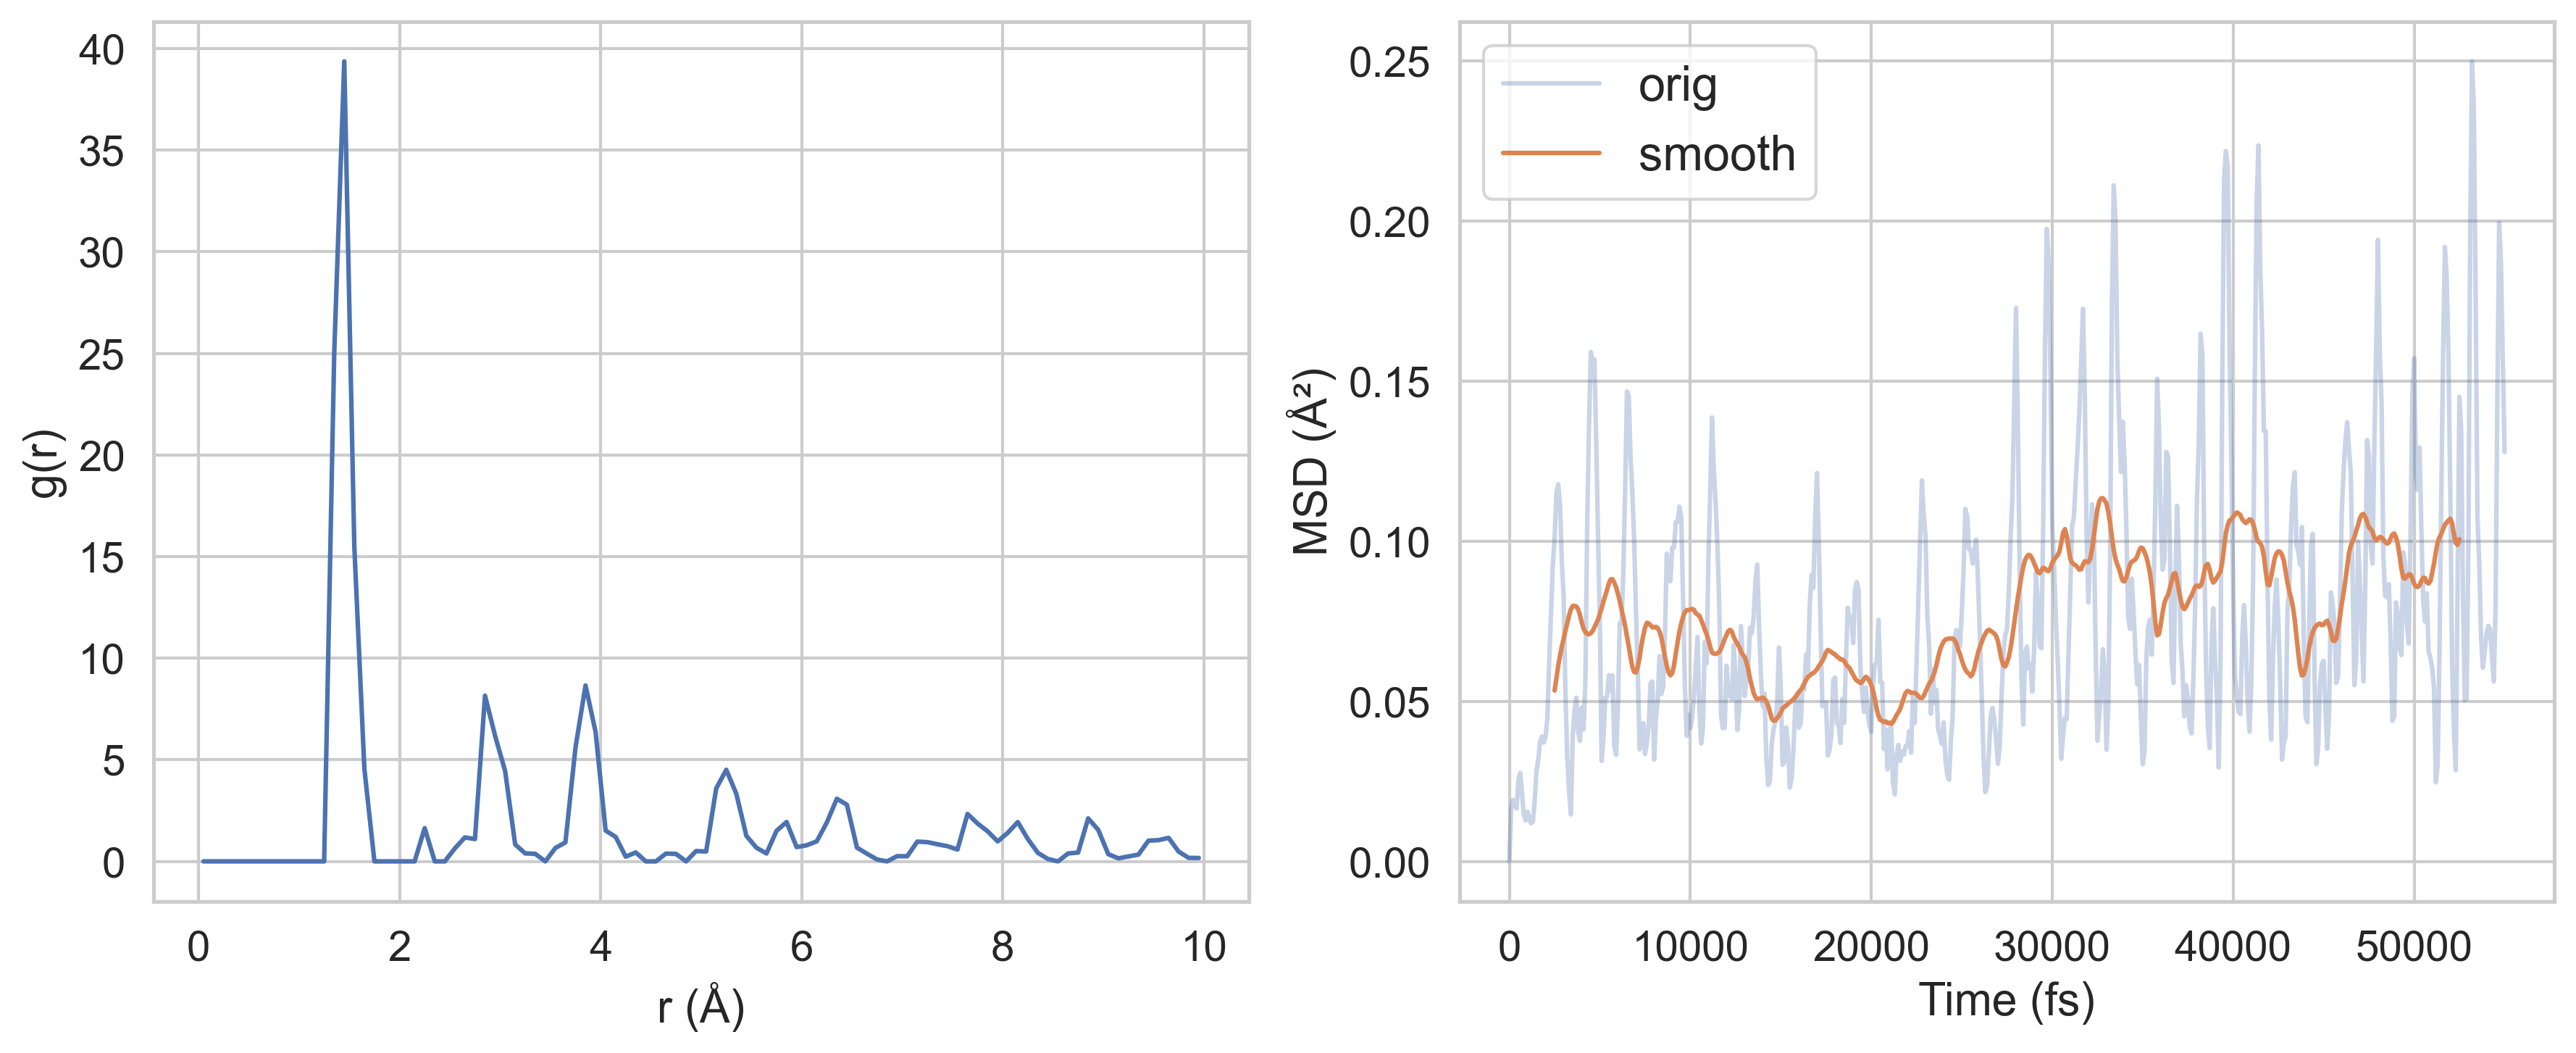
\includegraphics[width=\linewidth]{NN_1225K_notitle.png}
    \caption{Cacat N\textsubscript{B}, 1225 K}
    \label{subfig:rdf_msd_nn_1225k}
  \end{subfigure}
\end{figure}

% --- Bagian 3: Cacat B_N ---
\begin{figure}[H]\ContinuedFloat
  \centering
  \begin{subfigure}{0.9\textwidth}
    \centering
    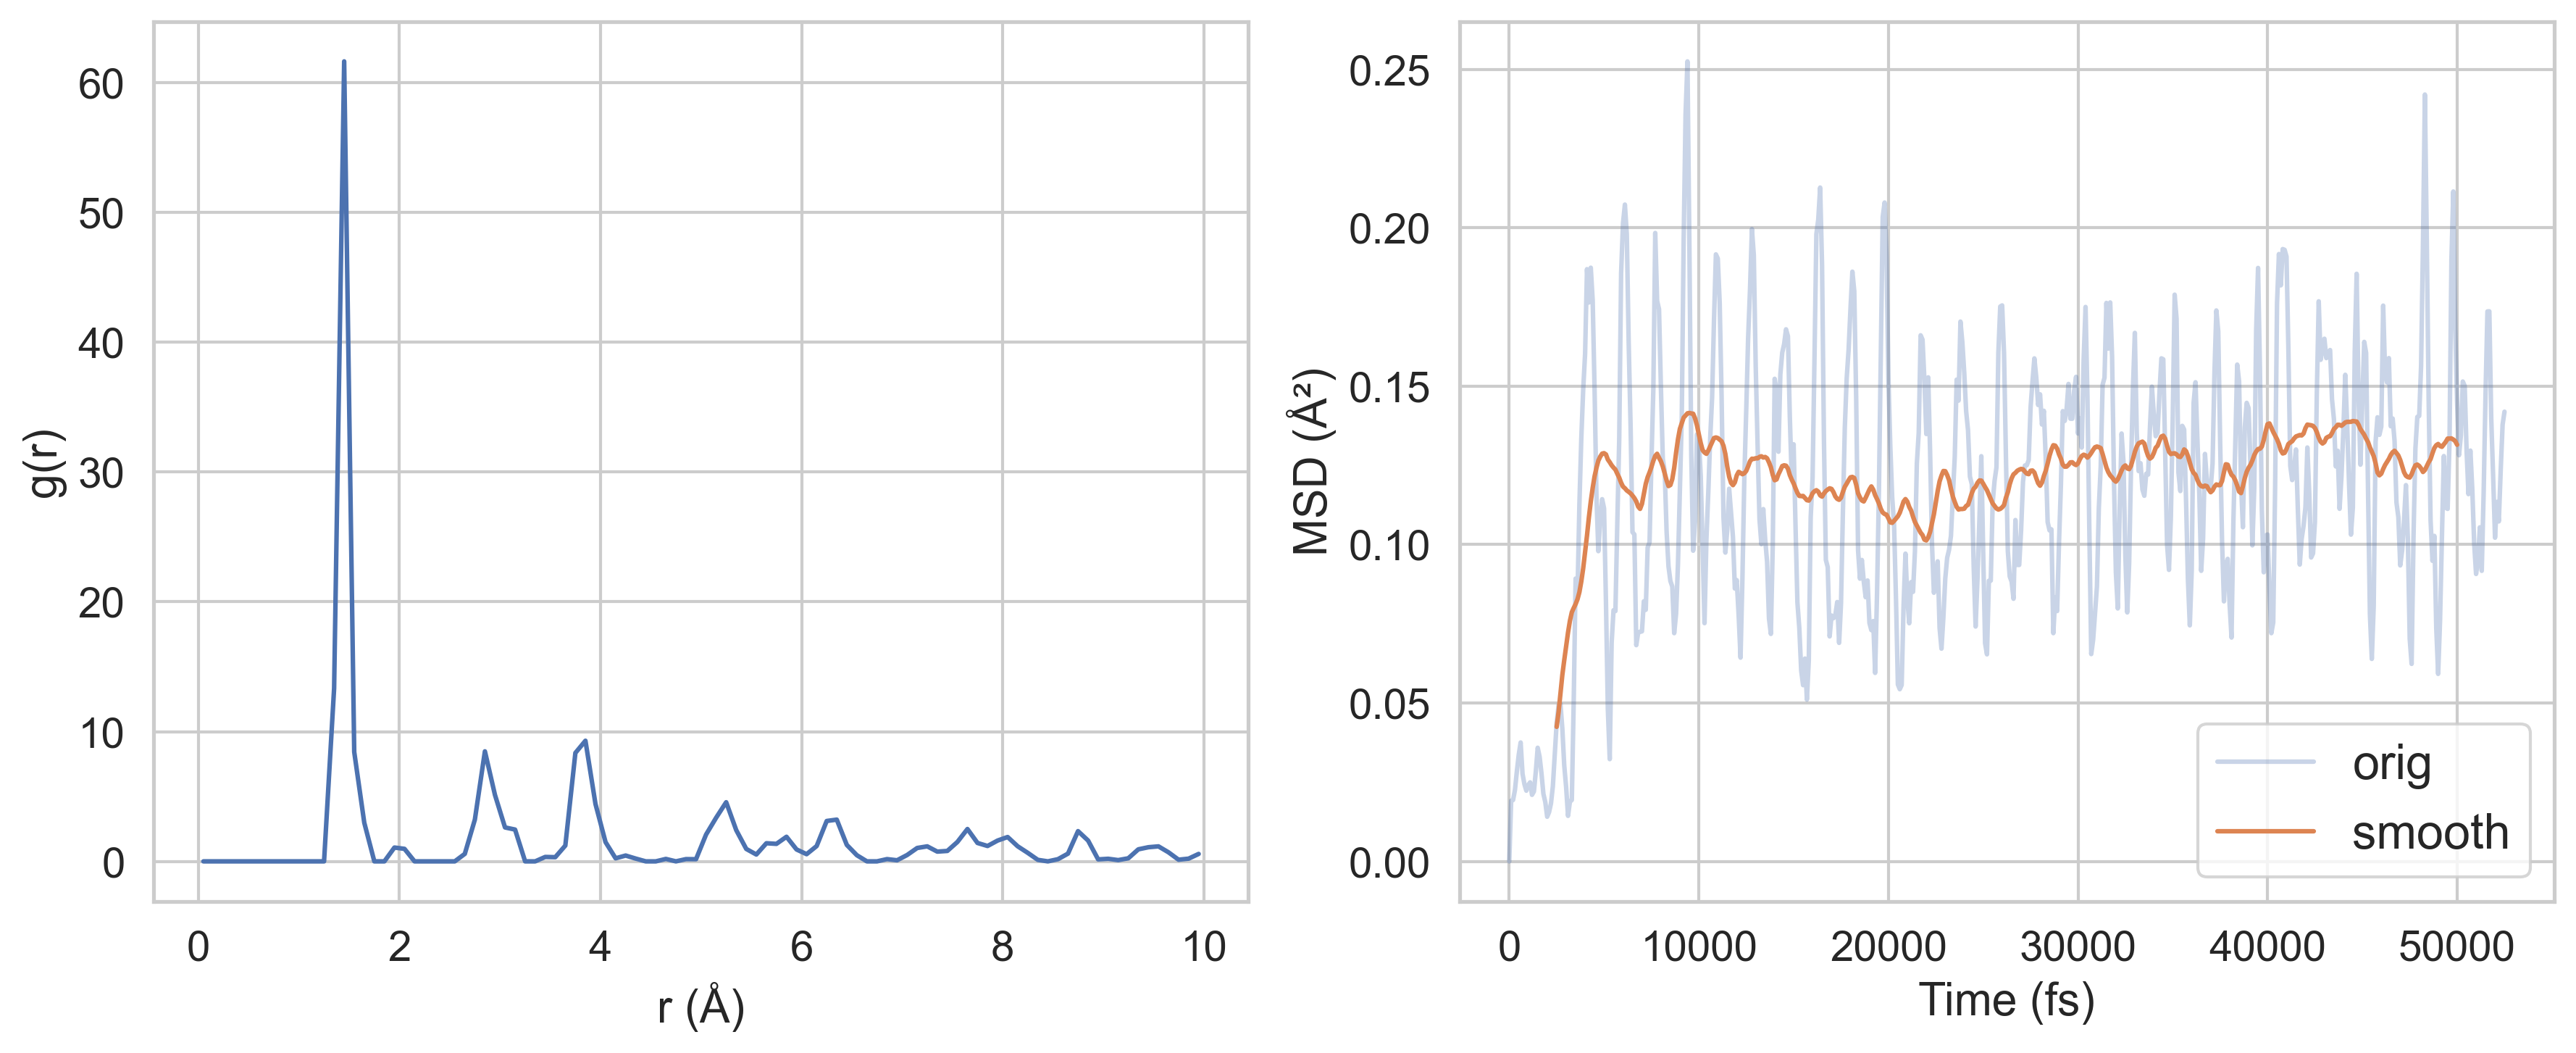
\includegraphics[width=\linewidth]{BB_800K_notitle.png}
    \caption{Cacat B\textsubscript{N}, 800 K}
    \label{subfig:rdf_msd_bb_800k}
  \end{subfigure}
  \vspace{1em}
  \begin{subfigure}{0.9\textwidth}
    \centering
    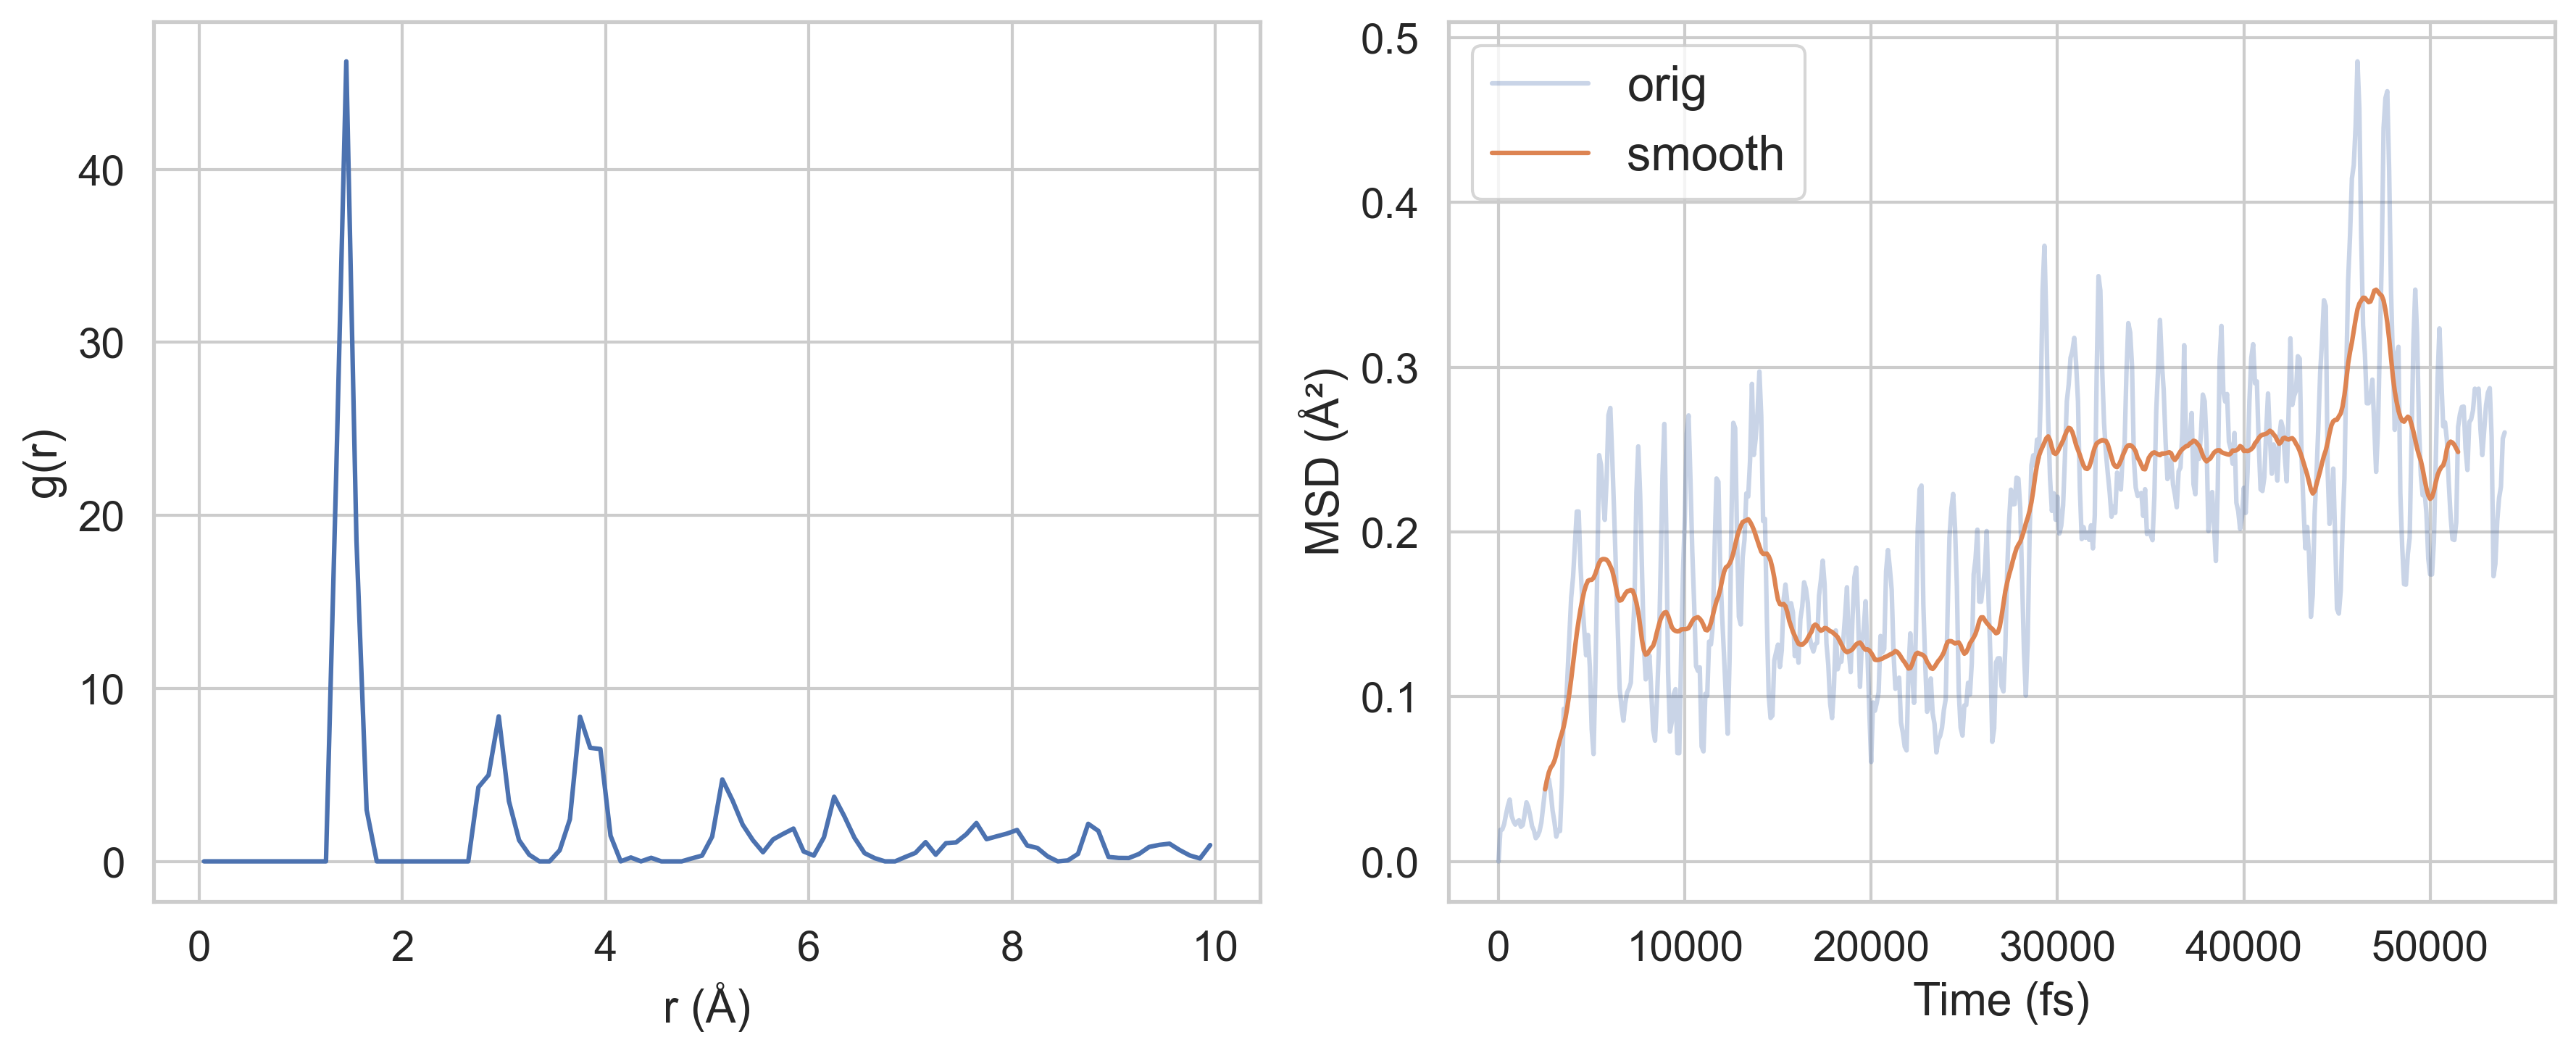
\includegraphics[width=\linewidth]{BB_1100K_notitle.png}
    \caption{Cacat B\textsubscript{N}, 1100 K}
    \label{subfig:rdf_msd_bb_1100k}
  \end{subfigure}
  \vspace{1em}
  \begin{subfigure}{0.9\textwidth}
    \centering
    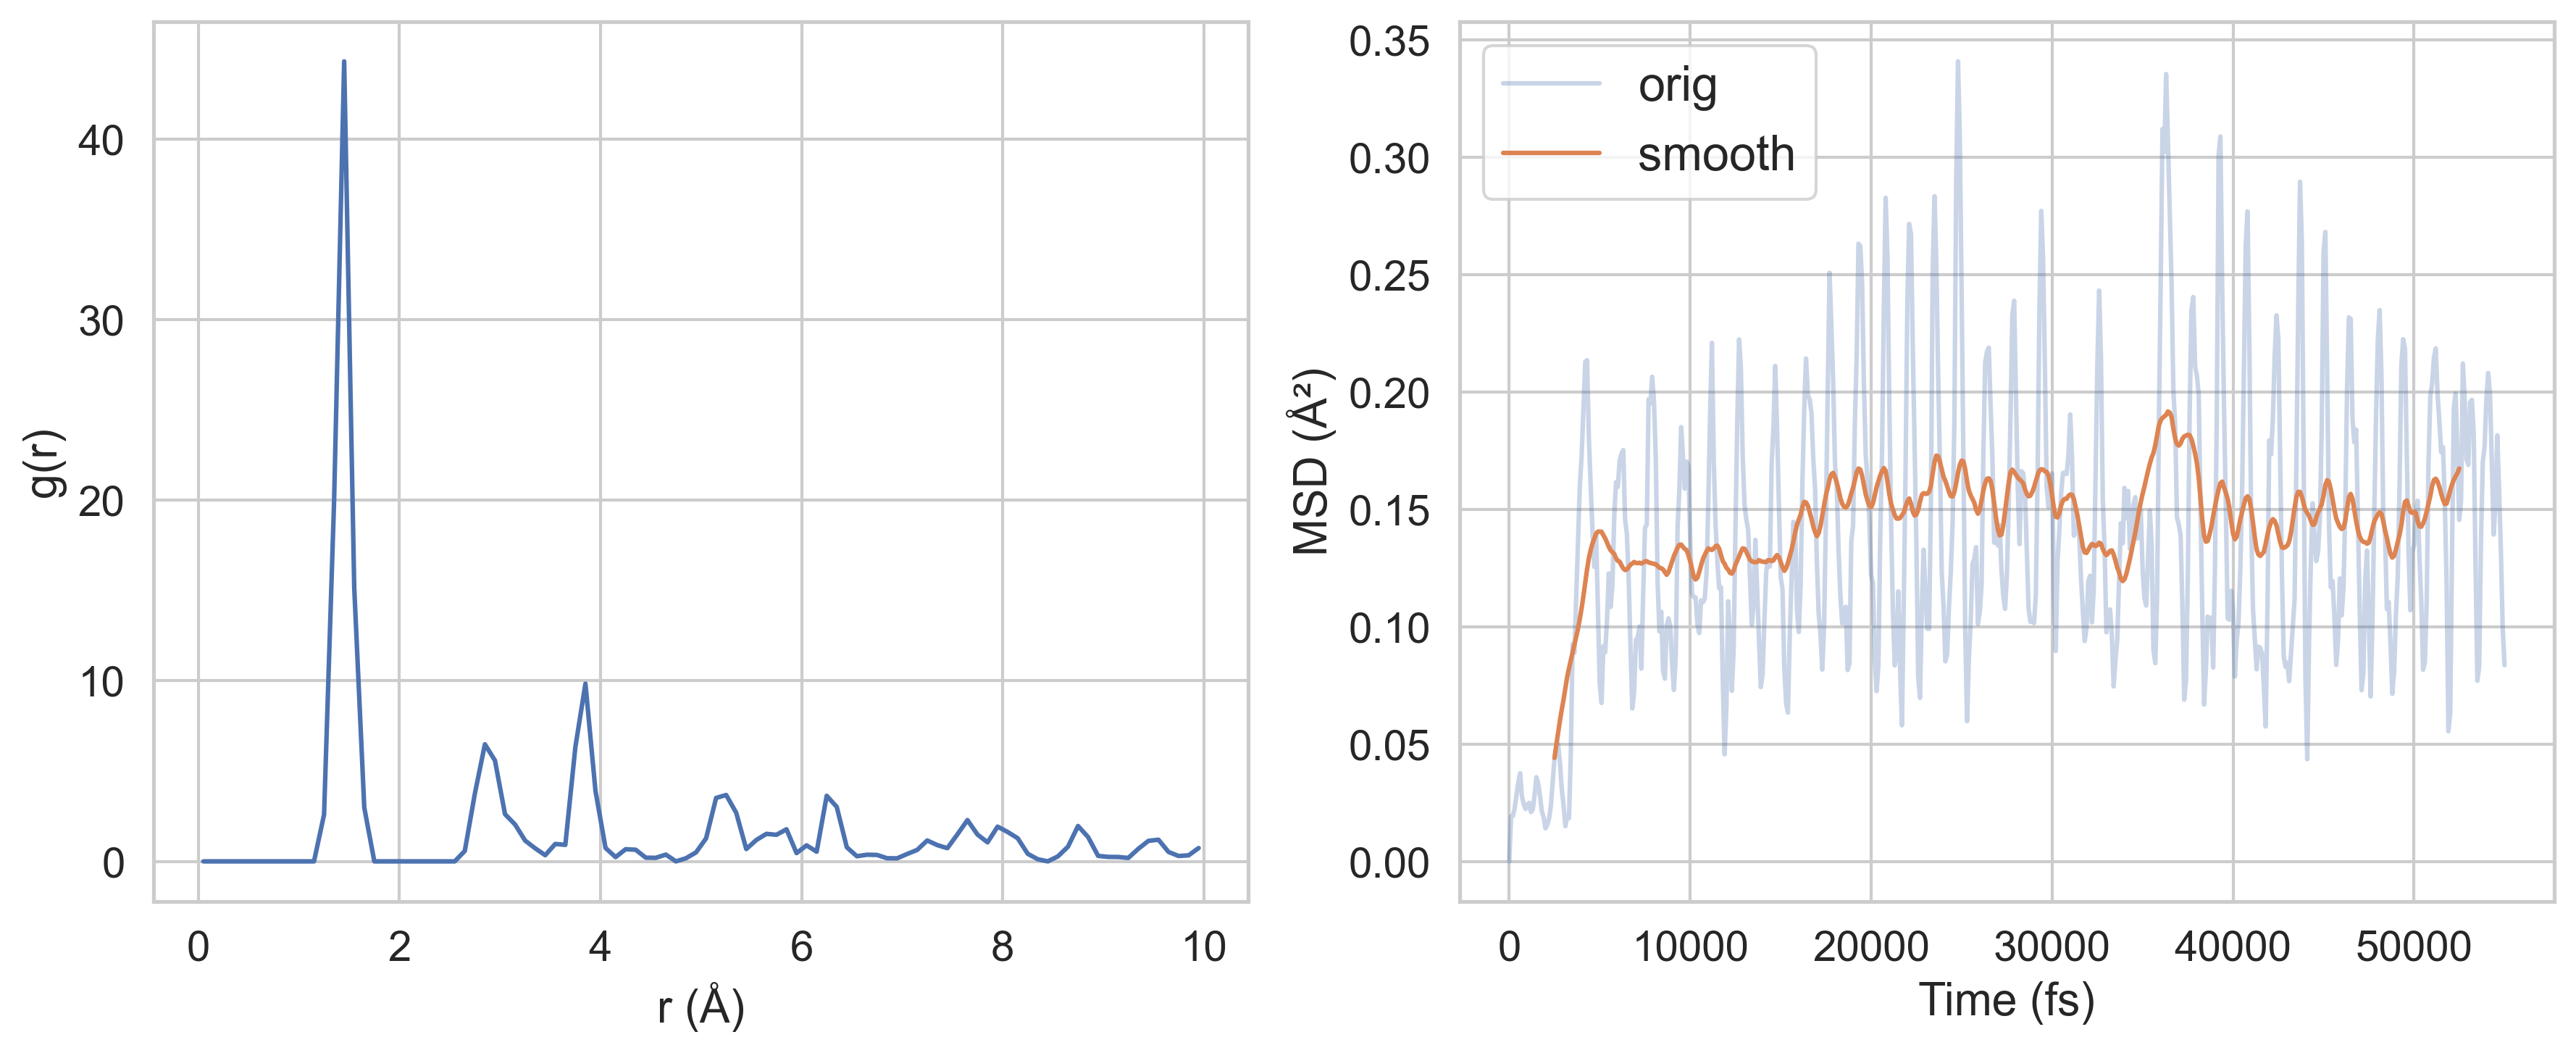
\includegraphics[width=\linewidth]{BB_1225K_notitle.png}
    \caption{Cacat B\textsubscript{N}, 1225 K}
    \label{subfig:rdf_msd_bb_1225k}
  \end{subfigure}
    \caption{Plot RDF dan MSD untuk setiap variasi}
\end{figure}
